\makeatletter
\newif\ifGm@compatii
\makeatother
\documentclass[12pt,landscape,english]{beamer}



\usepackage{bbding}
\usepackage{etoolbox, verbatim}

\usepackage{graphicx}
\graphicspath{{../figs/}}

%%%%%%%%%%%%%%%TIKZ

\usepackage{tikz}
\usetikzlibrary{positioning, fit,arrows,chains,shapes.geometric}
\usetikzlibrary{graphs,graphdrawing}
%\usetikzlibrary{decorations.text}
\usetikzlibrary{petri}
\usegdlibrary{force, layered, trees}
%%%%%%%%%%%%%%%%%%

%%%%%%%%%%%%%Bibliography
\usepackage[backend=bibtex, url=false,
bibstyle=ieee,firstinits=true]{biblatex}
\bibliography{../../../Resources/master_bibliography/master.bib}
\renewcommand*{\thefootnote}{} %No symbol or marker
\renewcommand{\footnotesize}{\scriptsize}
%%%%%%%%%%%%%%%%%




\mode<presentation>
%\setbeameroption{show notes}

%%%%%%%%%%%%%%%Template
\setbeamertemplate{navigation symbols}{}
\setbeamercolor{palette sidebar secondary}{fg=black,bg=blue!30!gray}
\setbeamercolor{sidebartitle}{fg=black,bg=blue!30!gray}
\useoutertheme{sidebar_custom}
\usebackgroundtemplate{\includegraphics[width=\paperwidth,height=\paperheight]{uwa_eng.png}}

\setbeamertemplate{itemize item}{\raisebox{-2px}{\JackStarBold} \hskip -.2em}
\setbeamertemplate{itemize subitem}{\raisebox{-2px}{\FourAsterisk} \hskip -.2em}
\setbeamertemplate{itemize subsubitem}{\raisebox{-2px}{\JackStar} \hskip -.2em}


\setbeamercolor{title}{fg=black}
\usefonttheme{structurebold}
\addtobeamertemplate{frametitle}{}{\vskip-1.2cm}

\setbeamercolor{sidebar}{fg=darkgray!80!black}

%%%%%%%%%%%%%%%%%%%%%%%%%%%%%%%%%%%


\makeatletter





\begin{document}
	
% Titlepage info

\title[Semantic Vectors]{Semantic Vector Representations for Natural Language}
\author[L.~White]{
	Lyndon White \texorpdfstring{\\\medskip{\scriptsize Supervised by:\\ Prof Roberto Togneri\\ Dr Wei Liu\\W/Prof Mohammed Bennamoun\\ }}{}}

\date{} % show no date
%\titlegraphic{\includegraphics[width=2.1cm]{balls}}

\begin{frame}[plain]
	\vfill
	\vspace{2cm}
	\titlepage
\end{frame}
}

%%%%%%%%%%%%%%%%%%%%Definitions

\def\x{\tilde{x}}
\def\y{\tilde{y}}
\def\b{\tilde{b}}


%%%%%%%%%%%%%%%%%%%%%%%%%%%%


\section{Introduction}
\begin{frame} {Natural Language} 
	
	\note{Shown are two lists of information. On one side are examples of informaition in a form easily accessable by software. On the other is information recored digitally in natural language.
		}
\begin{columns}[T]
	\begin{column}{0.5\textwidth}
		\centering\resizebox{0.4\textwidth}{!}{\includegraphics{pres/people.png}}
		\begin{itemize}
			\item $10^7$ {  StackOverflow QAs}
			\item $10^7$ Digitalised Books \note[item]{Google has digitalisd over 20 million books alone}
			\item $10^7$ Wikipedia Articles
			\item $10^8$ Amazon Reviews \note[item]{Amazon reviews from the Amazon Review dataset}
			\item $10^8$ Journal Articles \note[item]{Journal Articles from Web of Science extrapolated}
			\item ...

		\end{itemize}		
	\end{column}
		\begin{column}{0.5\textwidth}
			\centering\resizebox{0.4\textwidth}{!}{\includegraphics{pres/PC.png}}
			\begin{itemize}
				\item $10^6$ {  Cyc: Common- sense Facts}
				\item $10^6$ DBpedia Entries
				\item $10^8$ DNA Sequences \note[item]{GenBank Nucleotide}
%				\item $10^9$ Weather Records
				\item $10^{10}$ Census Records
				\item ...
			\end{itemize}		
		\end{column}
\end{columns}
	\note{NLU is the subarea of NLP which is base around creating software which in some sense comprehends the natural language.}
\end{frame}


\begin{frame} {Applications: Embeddings} 
		\vspace{1ex}
	\centering\resizebox{!}{0.5\textheight}{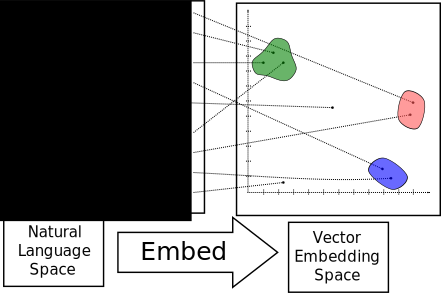
\includegraphics{./embed}}
	\vspace{1ex}
	\begin{itemize}
		\item Extractive Summarization
		\item Similarity Measurement \note{More over if the vector space can be made common between two languages, then we get biligaul sentence similarity, which has applications for machine translation.}
		\item Searching for Images with Descriptions \note{Historically Image search worked by looking for key words on a website and then returning that websites pictures. If we convert both the Embed both images and text to a common vector space then we can do similarity matching as just discussed}
		\item Feature Detector For Classifiers
		\note{\begin{itemize}
			\item Sentiment Analysis
			\item Topic Classification
			\item Paraphrase Detection
		\end{itemize}}
	\end{itemize}
\end{frame}

\begin{frame} {Applications: Full Cycle} 
	\centering\resizebox{!}{0.5\textheight}{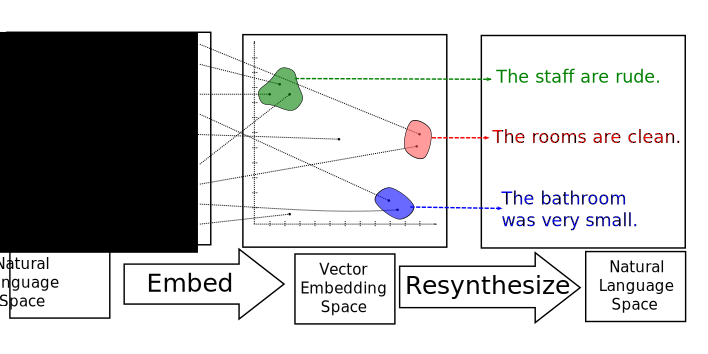
\includegraphics{./workflow}}
	\begin{itemize}
		\item Abstractive Summarization
		\item Paraphrase Generation \note{and this means using the multilanguage common vector space from before, Phrasal translation.}
		\item Generating Image Descriptions
		\item Semantically Lossy Text Compression \note{This is neat. Like a JPG image can be compressed by 2 orders of magnitude, at the cost of intoducting a few visual inaccuracies and blurs. We could compress text, at the cost of introducing artifacts in meaning.}
	\end{itemize}
\end{frame}


\section{Current Methods}
\begin{frame} {2 minute Intro To NNs}
	\begin{columns} 
	\begin{column}{0.5\textwidth}
		\centering\makeatletter
\tikz@def@grow@tokens{3}{1}{-1}{0}
\tikz@def@grow@tokens{3}{2}{0}{0}
\tikz@def@grow@tokens{3}{3}{1}{0}


\tikz@def@grow@tokens{5}{1}{-1}{0}
\tikz@def@grow@tokens{5}{2}{0}{0}
\tikz@def@grow@tokens{5}{3}{1}{0}
\tikz@def@grow@tokens{5}{4}{2}{0}
\tikz@def@grow@tokens{5}{5}{-2}{0}


\tikz@def@grow@tokens{7}{1}{-1}{0}
\tikz@def@grow@tokens{7}{2}{0}{0}
\tikz@def@grow@tokens{7}{3}{1}{0}
\tikz@def@grow@tokens{7}{4}{2}{0}
\tikz@def@grow@tokens{7}{5}{3}{0}
\tikz@def@grow@tokens{7}{6}{-2}{0}
\tikz@def@grow@tokens{7}{7}{-3}{0}
\makeatother

\begin{tikzpicture}[rotate=180,
sibling sep=20mm,level sep=10mm]
\def\x{\tilde{x}}
\def\a{\tilde{a}}
\def\y{\tilde{y}}
\def\b{\tilde{b}}
\def\tanh{\mathrm{tanh}}

\graph[layered layout, 
	edges={nodes={draw=none,minimum width=0mm, minimum height=0mm,
						 font=\scriptsize, inner sep=1pt}}
]{

	Input/""[draw, minimum width=1.6cm, rectangle,label=left:$\x$,label=right:Input, colored tokens={
lightgray,lightgray, black, lightgray,lightgray
}];

	hl/""[draw, minimum width=2.3cm, rectangle,
label=left:$\a$, label=right:Hidden, colored tokens={
lightgray,lightgray,gray, black, darkgray,gray,lightgray
}];
 	Output/""[draw, minimum width=1cm, rectangle,label=left:$\y$,label=right:Output, colored tokens={
lightgray, black, lightgray
}];

	Input->[edge label={$\sigma_1 \small(W_1\x+\b_1\small)$}] hl;
	hl ->[edge label={$\sigma_2 \small(W_2\a+\b_2\small)$}] Output;

};

\end{tikzpicture}
	\end{column}
	\begin{column}{0.5\textwidth}
	
			$f:\x\mapsto\y$
			$$NN\big(W_1,\b_1,..;\x\big)\approx f \big(\x\big)$$

		\colorbox{lime}{Tune:	$W_i,\b_i$}

	\end{column}
	\end{columns}
	\note[item]{But how to we get the vector representation $\x$ for the input in question?}
	\note[item]{Lets just assume we already knew it}
\end{frame}

\begin{frame} {NN with Embedding Look Up}
	\centering\resizebox{!}{0.7\textheight}{\makeatletter
\tikz@def@grow@tokens{3}{1}{-1}{0}
\tikz@def@grow@tokens{3}{2}{0}{0}
\tikz@def@grow@tokens{3}{3}{1}{0}


\tikz@def@grow@tokens{5}{1}{-1}{0}
\tikz@def@grow@tokens{5}{2}{0}{0}
\tikz@def@grow@tokens{5}{3}{1}{0}
\tikz@def@grow@tokens{5}{4}{2}{0}
\tikz@def@grow@tokens{5}{5}{-2}{0}


\tikz@def@grow@tokens{7}{1}{-1}{0}
\tikz@def@grow@tokens{7}{2}{0}{0}
\tikz@def@grow@tokens{7}{3}{1}{0}
\tikz@def@grow@tokens{7}{4}{2}{0}
\tikz@def@grow@tokens{7}{5}{3}{0}
\tikz@def@grow@tokens{7}{6}{-2}{0}
\tikz@def@grow@tokens{7}{7}{-3}{0}
\makeatother


\begin{tikzpicture}[word/.style={font=\itshape, label=below:Word Input},
	rec/.style={draw,rectangle},
 	xi/.style = {rec, minimum width=1.6cm},
   x1/.style = {xi, colored tokens={lightgray,lightgray, gray, lightgray,black}},
   x2/.style={xi, colored tokens={lightgray,lightgray, black, lightgray,lightgray}},
   x3/.style={xi, colored tokens={lightgray,gray, lightgray, black, lightgray}},
   x3_5/.style = {xi, colored tokens={black, gray,lightgray, gray, lightgray}},
   x4/.style={xi, colored tokens={gray,black, gray, lightgray,gray}},
   x5/.style={xi, colored tokens={gray,gray, black, lightgray,lightgray}},
]

\def\x{\tilde{x}}
\def\a{\tilde{a}}
\def\y{\tilde{y}}
\def\b{\tilde{b}}
\def\tanh{\mathrm{tanh}}


\node  (Iinf) [xi,label=left:$\x_{...}$] {...};
\node  (I5) [x5,label=left:$\x_{mat}$,below=0pt of Iinf] {};
\node  (I4) [x4,label=left:$\x_{on}$,below=0pt of I5] {};
\node  (I3_5) [x3_5,label=left:$\x_{fish}$,below=0pt of I4] {};
\node  (I3) [x3,label=left:$\x_{sat}$,below =0pt of I3_5] {};
\node  (I2) [x2,label=left:$\x_{cat}$,below =0pt of I3] {} ;
\node  (I1)[x1,label=left:$\x_{the}$,below = 0pt of I2] {};
\node  (I0)[xi,label=left:$\x_{...}$,below = 0pt of I1] {...};
\node (lookup_lbl)[font=\scriptsize, above = 0pt of Iinf, inner sep=1pt] {Lookup};
\node[blue, rounded corners, thick, line width=1pt, draw, fit = (I0) (lookup_lbl)] {};

\node  (J2) [x3,above right= 1.5cm of I3,label=left:$\x$, label=right:Word Embedding] {};
\draw[->] (I2.east) edge (J2);


\node  (W2) [word,below right= 1.5cm of I1] {Cat};
\draw[->] (W2) edge (I2.east);

\node (HL)[rec,  above = 1.5cm of J2, minimum width=2.3cm,  label=left:$\a$, label=right:Hidden,
					 colored tokens={lightgray,lightgray,gray, black, darkgray,gray,lightgray}]{};
\node (Output)[rec, above = 1.5cm of HL,  minimum width=1cm, label=left:$\y$,label=right:Output, 
							colored tokens={lightgray, black, lightgray}] {};
\draw[->] (J2) to node[left]{$\sigma_1 (W_1\x+\b_1)$} (HL) ;
\draw[->] (HL) to node[left]{$\sigma_2 (W_2\a+\b_2)$} (Output);




\end{tikzpicture}}
	
	\rightskip 1ex \colorbox{lime}{Tune:	$W_i,\b_i,\x_j$}
\end{frame}

\begin{frame} {Neural Probabalistic LM}
	\centering\resizebox{!}{0.7\textheight}{\makeatletter
\tikz@def@grow@tokens{3}{1}{-1}{0}
\tikz@def@grow@tokens{3}{2}{0}{0}
\tikz@def@grow@tokens{3}{3}{1}{0}


\tikz@def@grow@tokens{5}{1}{-1}{0}
\tikz@def@grow@tokens{5}{2}{0}{0}
\tikz@def@grow@tokens{5}{3}{1}{0}
\tikz@def@grow@tokens{5}{4}{2}{0}
\tikz@def@grow@tokens{5}{5}{-2}{0}


\tikz@def@grow@tokens{7}{1}{-1}{0}
\tikz@def@grow@tokens{7}{2}{0}{0}
\tikz@def@grow@tokens{7}{3}{1}{0}
\tikz@def@grow@tokens{7}{4}{2}{0}
\tikz@def@grow@tokens{7}{5}{3}{0}
\tikz@def@grow@tokens{7}{6}{-2}{0}
\tikz@def@grow@tokens{7}{7}{-3}{0}
\makeatother


\begin{tikzpicture}[word/.style={font=\itshape, label=below:Word Input},
	rec/.style={draw,rectangle},
 	xi/.style = {rec, minimum width=1.6cm},
   x1/.style = {xi, colored tokens={lightgray,lightgray, gray, lightgray,black}},
   x2/.style={xi, colored tokens={lightgray,lightgray, black, lightgray,lightgray}},
   x3/.style={xi, colored tokens={lightgray,gray, lightgray, black, lightgray}},
   x3_5/.style = {xi, colored tokens={black, gray,lightgray, gray, lightgray}},
   x4/.style={xi, colored tokens={gray,black, gray, lightgray,gray}},
   x5/.style={xi, colored tokens={gray,gray, black, lightgray,lightgray}},
   proc_word/.style={font=\large},
]

\def\x{\tilde{x}}
\def\a{\tilde{a}}
\def\y{\tilde{y}}
\def\b{\tilde{b}}
\def\tanh{\mathrm{tanh}}


\node  (Iinf) [xi,label=left:$\x_{...}$] {...};
\node  (I5) [x5,label=left:$\x_{mat}$,below=0pt of Iinf] {};
\node  (I4) [x4,label=left:$\x_{on}$,below=0pt of I5] {};
\node  (I3_5) [x3_5,label=left:$\x_{fish}$,below=0pt of I4] {};
\node  (I3) [x3,label=left:$\x_{sat}$,below =0pt of I3_5] {};
\node  (I2) [x2,label=left:$\x_{cat}$,below =0pt of I3] {} ;
\node  (I1)[x1,label=left:$\x_{the}$,below = 0pt of I2] {};
\node  (I0)[xi,label=left:$\x_{...}$,below = 0pt of I1] {...};
\node (lookup_lbl)[font=\scriptsize, above = 0pt of Iinf, inner sep=1pt] {Lookup};
\node[blue, rounded corners, thick, line width=1pt, draw, fit = (I0) (lookup_lbl)] {};

\node  (J1) [x1,above right= 1.5cm of I3,label=left:$\x$] {};
\node  (J2) [x2,right =0pt of J1] {} ;
\node  (J3)[x3, right = 0pt of J2, label=right: Concat'd] {};


\draw[->] (I1.east) edge (J1);
\draw[->] (I2.east) edge (J2);
\draw[->] (I3.east) edge (J3);

\node  (W1) [word,below right= 1.5cm of I1] {The};
\node  (W2) [word, right =1.3cm of W1] {Cat} ;
\node  (W3) [word, right = 1.3cm of W2] {Sat};
\draw[->] (W1) edge (I1.east);
\draw[->] (W2) edge (I2.east);
\draw[->] (W3) edge (I3.east);


\node (HL)[rec,  above = 1.5cm of J2, minimum width=2.3cm,  label=left:$\a$, label=right:Hidden,
					 colored tokens={lightgray,lightgray,gray, black, darkgray,gray,lightgray}]{};
\node (Output)[rec, above = 1.5cm of HL,  minimum width=1cm, label=left:$\y$,label=right:Next Word Prediction, 
							colored tokens={black, lightgray, lightgray}] {};
\node (pred) [below right = 3pt of Output,font=\itshape] {On};
\draw[->] (J2) to node[left]{$\sigma_1  (W_1\x+\b_1 )$} (HL) ;
\draw[->] (HL) to node[left]{$\sigma_2  (W_2\a+\b_2 )$} (Output);

%%%%%%%%%%%%%%%%%%%%

\node(inlbl)[proc_word, below=6cm of lookup_lbl]{\textbf{Process:}};
\node(wwThe1)[proc_word, right= 2ex of inlbl]{The};
\node(wwCat)[proc_word,right= 2ex of wwThe1]{Cat};
\node(wwSat)[proc_word,right= 2exof wwCat]{Sat};
\node(wwOn)[proc_word,right= 2ex of wwSat]{On};
\node(wwThe2)[proc_word,right= 2ex of wwOn]{The};
\node(wwMat)[proc_word,right= 2ex of wwThe2]{Mat};
\node(window)[draw, fit=(wwThe1)(wwSat), line width=1,green]{};
\node(pred)[draw, fit=(wwOn), line width=1,purple]{};




\end{tikzpicture}}
	\footfullcite{NPLM}
\end{frame}

\begin{frame} {Neural Probabalistic LM}
	\centering\resizebox{!}{0.7\textheight}{\input{../figs/NPLM2.pgf}}
	\footfullcite{NPLM}
\end{frame}

\begin{frame} {Neural Probabalistic LM}
	\centering\resizebox{!}{0.7\textheight}{\input{../figs/NPLM3.pgf}}
	\footfullcite{NPLM}
	
	\note{\begin{itemize}
		\item By tweaking this general structure we can produce a variety of models
		\item replace the simple classifier with a Convolutional Neural Net and share the word embedding look-up table across several tasks, and you get the Colbert and Weston Embeddings
		\item remove the hidden layer and average instead of concatenating and you get Continuous Bag of Word Embeddings
		\item make the task to use one word embedding to work out all the context works and you get Skip nGrams.
		\item There are a lot of word-embedding methods based on this idea
		
		\item That there is the limitation though, we get word embeddings, vector representations for the words. But most of the documents we want to use NLU  to understand are not words. They are sentences. Which is what the rest of this presentation will focus on.
		
		\item One issue is that we are not looking at all the content all the time. If a word at the start of a sentence has a lot of interaction with a word at the end, then the windowed model can't hand that.
		
		
		\end{itemize}

		}
	
	
\end{frame}


\begin{frame} {PV DM} 
	\centering\resizebox{!}{0.7\textheight}{\input{../figs/PVDM1.pgf}}
	\footfullcite{le2014distributed}
\end{frame}


\begin{frame} {PV DM} 
	\centering\resizebox{!}{0.7\textheight}{\input{../figs/PVDM2.pgf}}
	\footfullcite{le2014distributed}
\end{frame}


\begin{frame} {PV DM} 
	\centering\resizebox{!}{0.7\textheight}{\input{../figs/PVDM3.pgf}}
	\footfullcite{le2014distributed}
	
	\note[item]{This is a nice method. Now we have vectors for sentences, or paragraphs. As well as for words.}
\end{frame}


\begin{frame} {RvNN} 
	\centering\resizebox{!}{0.7\textheight}{\makeatletter
\tikz@def@grow@tokens{3}{1}{-1}{0}
\tikz@def@grow@tokens{3}{2}{0}{0}
\tikz@def@grow@tokens{3}{3}{1}{0}


\tikz@def@grow@tokens{5}{1}{-1}{0}
\tikz@def@grow@tokens{5}{2}{0}{0}
\tikz@def@grow@tokens{5}{3}{1}{0}
\tikz@def@grow@tokens{5}{4}{2}{0}
\tikz@def@grow@tokens{5}{5}{-2}{0}


\tikz@def@grow@tokens{7}{1}{-1}{0}
\tikz@def@grow@tokens{7}{2}{0}{0}
\tikz@def@grow@tokens{7}{3}{1}{0}
\tikz@def@grow@tokens{7}{4}{2}{0}
\tikz@def@grow@tokens{7}{5}{3}{0}
\tikz@def@grow@tokens{7}{6}{-2}{0}
\tikz@def@grow@tokens{7}{7}{-3}{0}
\makeatother

\begin{tikzpicture}[node distance=1cm,
	word/.style={font=\itshape},
	rec/.style={draw,rectangle},
	edge_square/.style={draw, rectangle,fill=cyan, font=\tiny},
 	xi/.style = {rec, minimum width=1.6cm},
   x1/.style = {xi, colored tokens={lightgray,lightgray, gray, lightgray,black}},
   x2/.style={xi, colored tokens={lightgray,lightgray, black, lightgray,lightgray}},
   x3/.style={xi, colored tokens={lightgray,gray, lightgray, black, lightgray}},
   x3_5/.style = {xi, colored tokens={black, gray,lightgray, gray, lightgray}},
   x4/.style={xi, colored tokens={gray,black, gray, lightgray,gray}},
   x5/.style={xi, colored tokens={gray,gray, black, lightgray,lightgray}},
%
    x10/.style={xi, colored tokens={lightgray,gray, gray, gray,lightgray}},
    x11/.style={xi, colored tokens={gray,lightgray, lightgray, lightgray,gray}},
    x12/.style={xi, colored tokens={gray,lightgray, gray, lightgray,gray}},
    x13/.style={xi, colored tokens={gray,black, gray, lightgray,gray}},
    x14/.style={xi, colored tokens={gray,lightgray, black, lightgray,gray}},
]

\def\x{\tilde{x}}
\def\a{\tilde{a}}
\def\y{\tilde{y}}
\def\b{\tilde{b}}
\def\tanh{\mathrm{tanh}}


\node  (JThe2) [x1] {};
\node  (JMat) [x5,right = 0pt of JThe2] {};
\node (JTheMat)[x11, above = of JThe2.east,xshift=-0.5cm]{};
\draw [->] (JThe2.east) to (JTheMat);


\node  (JOnTheMat) [x12, above= of JTheMat.west, xshift=-1cm] {};
\node  (JOn) [x4,left = 0pt of JTheMat] {};
\draw [->] (JTheMat.west) to (JOnTheMat);

\node (JSatOnTheMat)[x13, above= of JOnTheMat.west, xshift=-2cm]{};
\node  (JSat) [x3,left = 0pt of JOnTheMat] {};
\draw [->] (JOnTheMat.west) to (JSatOnTheMat);

\node (JTheCatSatOnTheMat)[x14, above= of JSatOnTheMat.west, label=right:Sentence Embedding]{};
\node (JTheCat)[x10, left =0pt of JSatOnTheMat]{};
\draw [->] (JSatOnTheMat.west) to (JTheCatSatOnTheMat);

\node  (JThe1) [x1, below = of JTheCat.west,xshift=-2cm] {};
\node  (JCat) [x2, right = 0pt of JThe1] {};
\draw [->] (JThe1.east) to (JTheCat);



\node  (WThe1) [word, below = 2cm of JThe1] {The};
\node  (WCat) [word, below = 2cm of JCat] {Cat};
\node  (WSat) [word, below =3cm of JSat] {Sat};
\node  (WOn) [word, below = 2cm of JOn] {On};
\node  (WThe2) [word, below = of JThe2] {The};
\node  (WMat) [word, below = of JMat] {Mat};


\foreach \name in {The1, Cat, Sat, On, The2, Mat}
{
	\draw[->] (W\name) to node[edge_square]{--} (J\name);
}


\node (legend_square) [edge_square]{--};






\end{tikzpicture}}
	\note[item]{ constituency-based parse tree, Not Reoccurant}
	\note[item]{Here is an alternitive, the Recurssive Neural Net, merges its inputs, pairwise in a tree}
	\note[item]{At each level we get a new embedding. Which is concatenated with another and merged again until we reach the top}
	\note[item]{It reuses the same embedding matrix}
	\note[item]{In the black box can go more or less anything, probably a more traditional neural network classifier, so long as it produces a error signal which can be backproperated.}
	\footfullcite{socher2010PhraseEmbedding}
\end{frame}

\begin{frame} {URAE}
		\vskip 2ex
		\centering\resizebox{!}{0.8\textheight}{\input{../figs/URAE.pgf}}
		\footfullcite{SocherEtAl2011:PoolRAE}
\end{frame}

\begin{frame} {Semisupervised URAE} 
		\vskip 2ex
		\centering\resizebox{!}{0.8\textheight}{\makeatletter
\tikz@def@grow@tokens{3}{1}{-1}{0}
\tikz@def@grow@tokens{3}{2}{0}{0}
\tikz@def@grow@tokens{3}{3}{1}{0}


\tikz@def@grow@tokens{5}{1}{-1}{0}
\tikz@def@grow@tokens{5}{2}{0}{0}
\tikz@def@grow@tokens{5}{3}{1}{0}
\tikz@def@grow@tokens{5}{4}{2}{0}
\tikz@def@grow@tokens{5}{5}{-2}{0}


\tikz@def@grow@tokens{7}{1}{-1}{0}
\tikz@def@grow@tokens{7}{2}{0}{0}
\tikz@def@grow@tokens{7}{3}{1}{0}
\tikz@def@grow@tokens{7}{4}{2}{0}
\tikz@def@grow@tokens{7}{5}{3}{0}
\tikz@def@grow@tokens{7}{6}{-2}{0}
\tikz@def@grow@tokens{7}{7}{-3}{0}
\makeatother

\begin{tikzpicture}[node distance=1cm,
	word/.style={font=\itshape},
	rec/.style={draw,rectangle},
	edge_square/.style={draw, rectangle,fill=cyan, font=\tiny},
	edge_circle/.style={draw, circle,fill=pink, font=\tiny},
	edge_circle_un/.style={draw, circle,fill=yellow!40, font=\tiny},
	unfold/.style={},
 	xi/.style = {rec, minimum width=1.6cm},
   x1/.style = {xi, colored tokens={lightgray,lightgray, gray, lightgray,black}},
   x2/.style={xi, colored tokens={lightgray,lightgray, black, lightgray,lightgray}},
   x3/.style={xi, colored tokens={lightgray,gray, lightgray, black, lightgray}},
   x3_5/.style = {xi, colored tokens={black, gray,lightgray, gray, lightgray}},
   x4/.style={xi, colored tokens={gray,black, gray, lightgray,gray}},
   x5/.style={xi, colored tokens={gray,gray, black, lightgray,lightgray}},
%
    x10/.style={xi, colored tokens={lightgray,gray, gray, gray,lightgray}},
    x11/.style={xi, colored tokens={gray,lightgray, lightgray, lightgray,gray}},
    x12/.style={xi, colored tokens={gray,lightgray, gray, lightgray,gray}},
    x13/.style={xi, colored tokens={gray,black, gray, lightgray,gray}},
    x14/.style={xi, colored tokens={gray,lightgray, black, lightgray,gray}},
]

\def\x{\tilde{x}}
\def\a{\tilde{a}}
\def\y{\tilde{y}}
\def\b{\tilde{b}}
\def\tanh{\mathrm{tanh}}


\node  (JThe2) [x1] {};
\node  (JMat) [x5,right = 0pt of JThe2] {};
\node (JTheMat)[x11, above = of JThe2.east,xshift=-0.5cm]{};
\draw [->] (JThe2.east) to node[edge_circle]{} (JTheMat);


\node  (JOnTheMat) [x12, above= of JTheMat.west, xshift=-1cm] {};
\node  (JOn) [x4,left = 0pt of JTheMat] {};
\draw [->] (JTheMat.west) to node[edge_circle]{} (JOnTheMat);

\node (JSatOnTheMat)[x13, above= of JOnTheMat.west, xshift=-2cm]{};
\node  (JSat) [x3,left = 0pt of JOnTheMat] {};
\draw [->] (JOnTheMat.west) to node[edge_circle]{} (JSatOnTheMat);

\node (JTheCatSatOnTheMat)[x14, above= of JSatOnTheMat.west,label=right:Sentence Embedding]{};
\node (JTheCat)[x10, left =0pt of JSatOnTheMat]{};
\draw [->] (JSatOnTheMat.west) to node[edge_circle]{} (JTheCatSatOnTheMat);

\node  (JThe1) [x1, below = of JTheCat.west,xshift=-2cm] {};
\node  (JCat) [x2, right = 0pt of JThe1] {};
\draw [->] (JThe1.east) to node[edge_circle]{} (JTheCat);



\node  (WThe1) [word, below = 2cm of JThe1] {The};
\node  (WCat) [word, below = 2cm of JCat] {Cat};
\node  (WSat) [word, below =3cm of JSat]{Sat};
\node  (WOn) [word, below = 2cm of JOn] {On};
\node  (WThe2) [word, below = of JThe2] {The};
\node  (WMat) [word, below = of JMat] {Mat};


\foreach \name in {The1, Cat, Sat, On, The2, Mat}
{
	\draw[->] (W\name) to node[edge_square]{--} (J\name);
}



\node (black_box) [draw=none, minimum height=1.5cm, minimum width=1.5cm, above = of JTheCatSatOnTheMat] {};
\draw[->] (JTheCatSatOnTheMat) to node[edge_circle_un]{} (black_box);

\node (black_box2) [draw, dashed, cloud,cloud puffs=10.8,cloud puff arc=120, cloud ignores aspect, fill=green!70!brown!50,xshift=4.5cm, above right = of JTheCatSatOnTheMat, align=center] {Sub-network\\Performing\\Useful Task};

\draw[->] (JTheCatSatOnTheMat) to node[]{} (black_box2);



\node  (JTThe2) [x1, unfold, yshift=9.2cm] {}; %%%%%%%%%%%%%%%%%%%%%%%%%%%%%%%%%%%%%CHANGE THIS YSHIFT
\node  (JTMat) [x5,right = 0pt of JTThe2, unfold] {};
\node (JTTheMat)[x11, below = of JTThe2.east,xshift=-0.5cm, unfold]{};
\draw [<-, unfold] (JTThe2.east) to node[edge_circle_un]{} (JTTheMat);


\node  (JTOnTheMat) [x12, below= of JTTheMat.west, xshift=-1cm, unfold] {};
\node  (JTOn) [x4,left = 0pt of JTTheMat, unfold] {};
\draw [<-, unfold] (JTTheMat.west) to node[edge_circle_un]{} (JTOnTheMat);

\node (JTSatOnTheMat)[x13, below= of JTOnTheMat.west, xshift=-2cm, unfold]{};
\node  (JTSat) [x3,left = 0pt of JTOnTheMat, unfold] {};
\draw [<-, unfold] (JTOnTheMat.west) to node[edge_circle_un]{} (JTSatOnTheMat);

%\node (JTTheCatSatOnTheMat)[x14, below= of JTSatOnTheMat.west, label=right:Sentence Embedding, unfold]{};
\node (JTTheCat)[x10, left =0pt of JTSatOnTheMat, unfold]{};
%\draw [<-, unfold] (JTSatOnTheMat.west) to node[edge_circle_un]{} (JTTheCatSatOnTheMat);

\node  (JTThe1) [x1, above = of JTTheCat.west,xshift=-2cm, unfold] {};
\node  (JTCat) [x2, right = 0pt of JTThe1, unfold] {};
\draw [<-,unfold] (JTThe1.east) to node[edge_circle_un]{} (JTTheCat);



\node  (WTThe1) [word, above = 2cm of JTThe1, unfold] {The};
\node  (WTCat) [word, above = 2cm of JTCat, unfold] {Cat};
\node  (WTSat) [word, above =3cm of JTSat, unfold]{Sat};
\node  (WTOn) [word, above = 2cm of JTOn, unfold] {On};
\node  (WTThe2) [word, above = of JTThe2, unfold] {The};
\node  (WTMat) [word, above = of JTMat, unfold] {Mat};


\foreach \name in {The1, Cat, Sat, On, The2, Mat}
{
	\draw[<-, unfold] (WT\name) to node[edge_square]{--} (JT\name);
}



\node (legend_square) [edge_square, yshift=1.0cm, left = 6.2cm of JTheCatSatOnTheMat]{--};
\node (legend_circle) [edge_circle, below= 2ex of legend_square]{};
\node (legend_circle_un) [edge_circle_un, below= 2ex of legend_circle]{};
\node (lbl_square) [right = 6pt of legend_square] {Via Lookup Table};
\node (lbl_circle) [right = 6pt of legend_circle] {$\sigma(W_{fold}\x+\b_{fold})$};
\node (lbl_circle_un) [right = 6pt of legend_circle_un] {$\sigma(W_{unfold}\x+\b_{unfold})$};

\node[draw, rounded corners, dashed, orange, fit = (legend_circle) (legend_square) (lbl_square) (lbl_circle)(lbl_circle_un)] {};





\end{tikzpicture}}
		\footfullcite{zhang2014BRAE}
\end{frame}

\section{Future Work}
\begin{frame}{Not reversible}
	Even The URAE which looks reversible, requires you to know the way out to get there.
	For RvNN decended models, we end up with a tree search problem
\end{frame}

\begin{frame}{Not semantic, enough}
	
	S/MOWE
	BRAE
\end{frame}


\section{Conclusion}
\begin{frame}{Conclusion: There}
	\begin{itemize}
		\item Too much information for people to handle
		\item but written only for people
		\item need to make machines handle Natural Language
		\item machine are good at numbers
		\item so we turn sentences into numbers.
	\end{itemize}
\end{frame}

\begin{frame}{Conclusion: and Back Again}
	\begin{itemize}
		\item Once they are vectors, operate on them
		\item Go back to sentences
		\item to go back to sentences, position needs to corespond to meaning
		\item and must have method to get back
	\end{itemize}
\end{frame}


	


\end{document}
